\documentclass[en]{../../../../../../eplexam}

\usepackage{../../../../../../eplunits}
\usepackage[american]{circuitikz}
\usepackage{bm}

\hypertitle{Power Electronics}{7}{ELEC}{2660}{2019}{Janvier}{All}
{Martin Braquet \and Louis Fichefet \and Clément Martin}
{Marc Bekemans}

\section{Expliquez ce slide (contexte, explications détaillées, équations, \dots)  /4}

\begin{figure}[h!]
    \centering
    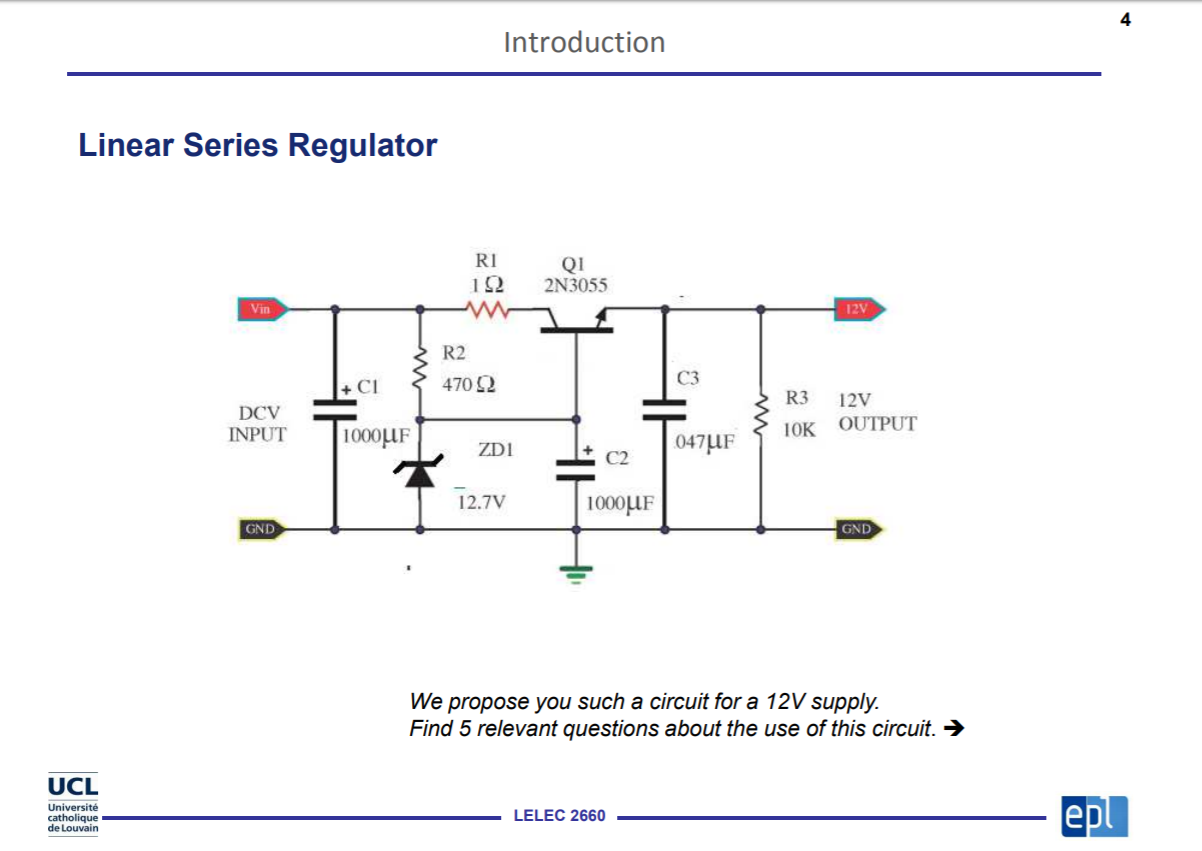
\includegraphics[scale=0.5]{Q1.png}
\end{figure}

\nosolution

\section{Expliquez ce slide (contexte, explications détaillées, équations,\dots)  /4}

\begin{figure}[h!]
    \centering
    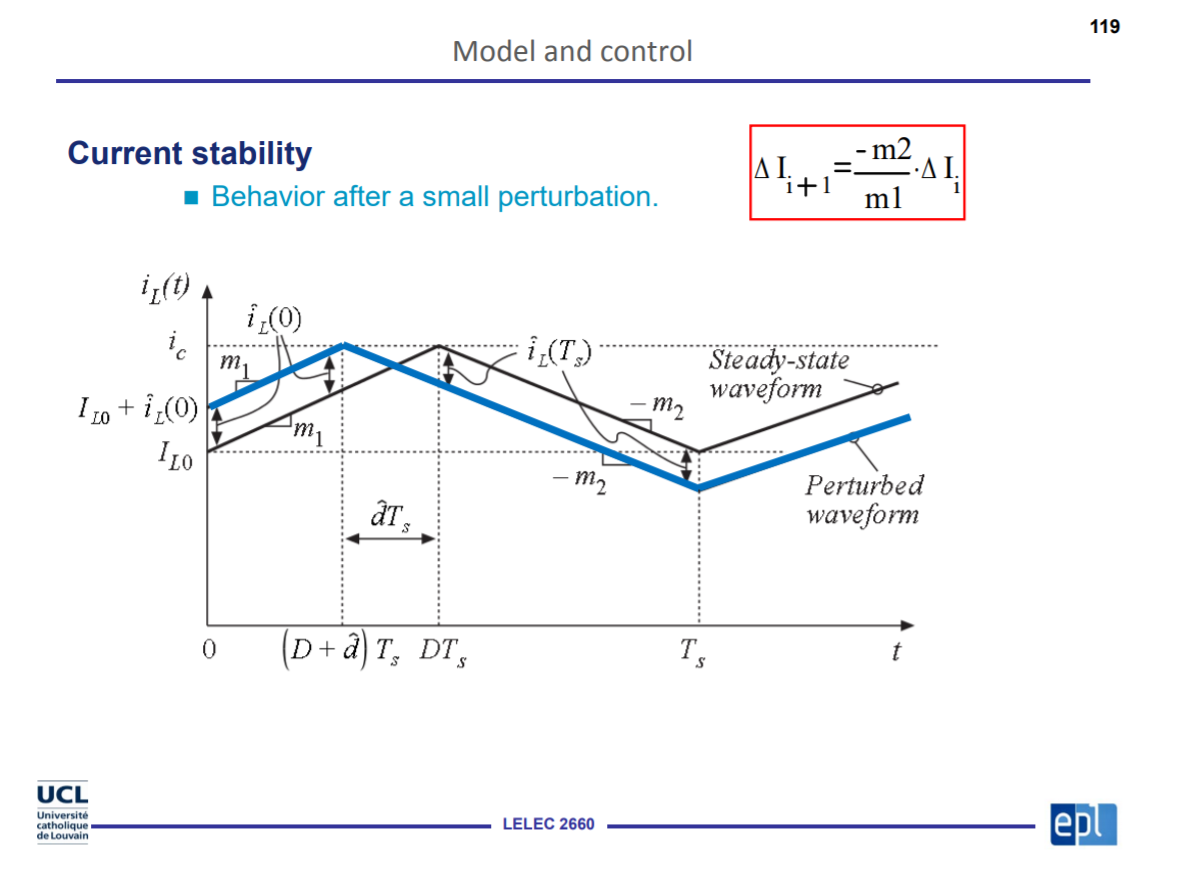
\includegraphics[scale=0.5]{Q2.png}
\end{figure}

\nosolution

\section{Série de questions rapides  /16}

\begin{itemize}
    \item En mode bloqué, un IGBT bloque les tensions dans les deux sens. Vrai/Faux.
    \item Soit un convertisseur Flyback. Quelles sont les conséquences au fait de doubler l'entrefer ?
    \item Soit un redresseur en bialternance connecté à une charge résistive avec une tension de 50 V DC à ses bornes. On décide de remplacer la charge par une capacité. Quelle est la tension à ses bornes ?
    \item Soit un redresseur triphasé non commandé à 6 diodes et alimenté par du 50 Hz. Quelle est la fréquence de la fondamentale de la tension de sortie ?
    \item Dans le peak current control, la condition de stabilité est que le rapport cyclique ne dépasse pas 50 \%. Vrai/Faux.
    \item Une diode avec les caractéristiques suivantes : $V_f = 850$ mV, $R_{th_{j-C}}$ = 0.15 K/W est parcourue par un courant de 50 A pendant 30 \% du temps sur une période. Sachant que l'air ambiant est à \SI{25}{\celsius} et que la température de jonction de la diode ne peut pas dépasser \SI{100}{\celsius}, quelle doit être la résistance thermique du radiateur ?
    \item Soit un convertisseur Buck avec les caractéristiques suivantes : $V_o$ = 25 V, $V_i$ = 100 V, $f_{SW} = \SI{100}{kHz}$, $L = \SI{250}{\micro H}$, quelle est la puissance de sortie minimale requise ?
    \item Écrivez l'équation du transfert de puissance complexe entre deux sources de courant alternatives $U_1$ et $U_2$ liées par une inductance $L$.
\end{itemize}

\begin{solution}
  \begin{itemize}
  \item Vrai
  \item Permet de doubler le courant, sans rentrer dans la zone de saturation magnétique.
  \item 50 V
  \item 2*3*50 = 300 Hz
  \item Vrai
  \item Il n'y a pas besoin de radiateur 
  $$\Delta T = R_{thj-c} * V * I_{avg} = 0.15*0.85*50*0.3 = \SI{1.9}{\celsius}$$
  $$T_{max} - \Delta T - T_a = \Delta T_{r} = \SI{73.1}{\celsius}$$
  $$R_r = \frac{\Delta T_r}{P} = \SI{5.73}{\celsius\per\watt}$$
\item 
  $$\theta = \frac{25}{100} = 0.25$$
$$R \leq \frac{2Lf}{1-\theta} = \SI{66.6}{\ohm}$$
  $$P = \frac{V^2}{R} = \SI{9.38}{\watt}$$
\item $$S_1 = \frac{U_1U_2}{\omega L}\sin(\alpha) + j \left(\frac{U_1U_2}{\omega L} \cos(\alpha) - \frac{U_1^2}{\omega L}\right)$$
  \end{itemize}
\end{solution}
\section{Exercice  /4}

On considère un Boost avec les caractéristiques suivantes :
\begin{itemize}
    \item $V_{in}$ = 50 V
    \item $V_{out}$ = 100 V
    \item $L = \SI{500}{\micro H}$
    \item $f_{sw}$ = 100 kHz
    \item $P_{out}$ = 100 W
\end{itemize}
Déterminez le nombre de capacités ($C = \SI{100}{\micro F}$, $r = \SI{100}{m\Omega}$) mises en sortie pour que le ripple de la tension de sortie ne dépasse pas $150$ mV (peak to peak).

\begin{solution}
On va approximer le ripple maximum par
$$\max(\Delta u) = \max(\Delta u_r) + \max(\Delta u_c) $$
$$\max(\Delta u_r) = r (i_{c,max} - i_{c,min}) = r\left(\frac{i_{ch}}{1-\theta} + \frac{\Delta i}{2} \right)$$
$$\max(\Delta u_c) = \frac{\theta T i_{ch}}{C}$$
$$\Delta i = \frac{E\theta T}{L}$$
$$i_{ch} = \SI{1}{\ampere}$$
En mettant les capacités en parallèle, on va diviser r par n, et multiplier C par n
$$\frac{r\left(\cfrac{i_{ch}}{1-\theta} + \frac{\Delta i}{2} \right) + \cfrac{\theta T i_{ch}}{C}}{\max(\Delta U)} \leq n$$
 $$1.83 \leq n$$
 On doit mettre 2 capacités en parallèle. (Rmq: sans la résistance, une seule capacité aurait suffit).
\end{solution}

\section{Question de théorie  /6}
    
On considère ici un convertisseur Flyback dans lequel on a rajouté un \textit{snubber}\footnote{Le \textit{snubber} a été vu en séance d'exercice sous la forme d'un projet dédié à la conception d'un transformateur.}. Expliquez le fonctionnement du snubber et comment choisir ses composants. Commentez, dessinez les formes d'ondes, schémas, etc.

\begin{solution}
Le snubber permet d'éviter le pic de tension dû à l'inductance de fuite. Nous avons besoin de réduire ce pic de tension pour protéger le transistor.

On va retrouver une évolution différentes des courants dans le transformateur et de la tension aux bornes du transistor.

\begin{figure}[H]
\centering
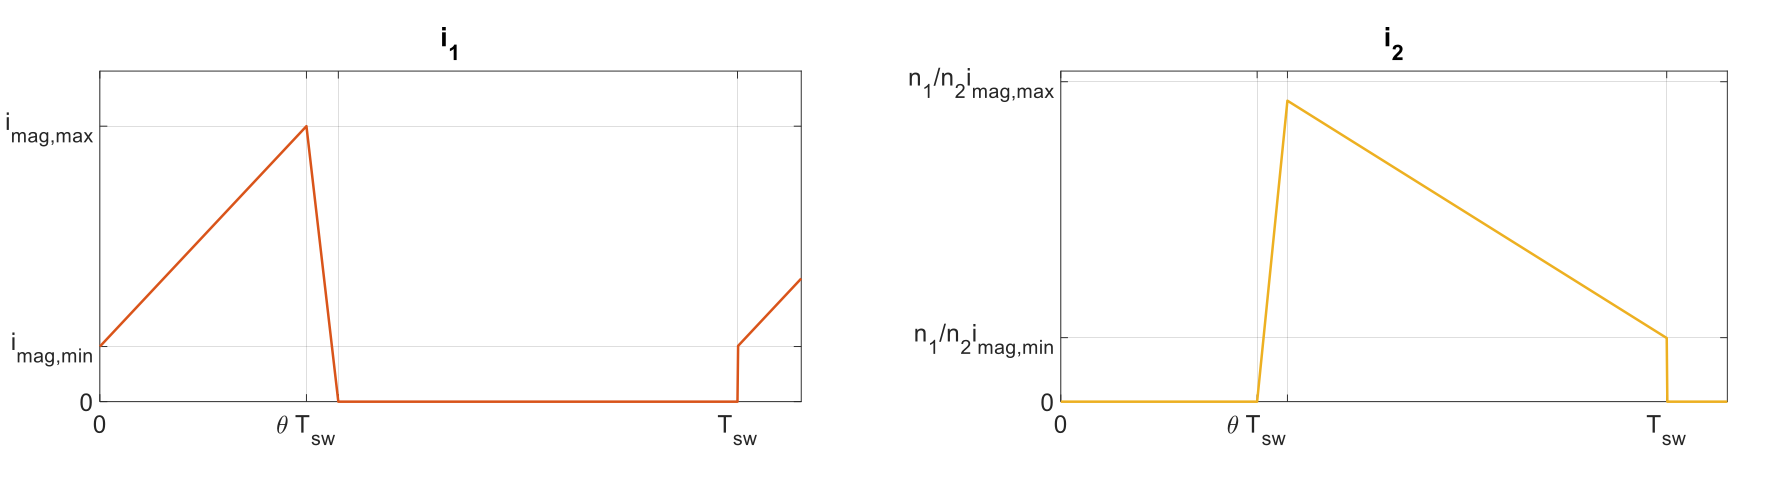
\includegraphics[width=\textwidth]{Snubber1.png}
\end{figure}

\begin{figure}[H]
  \centering
  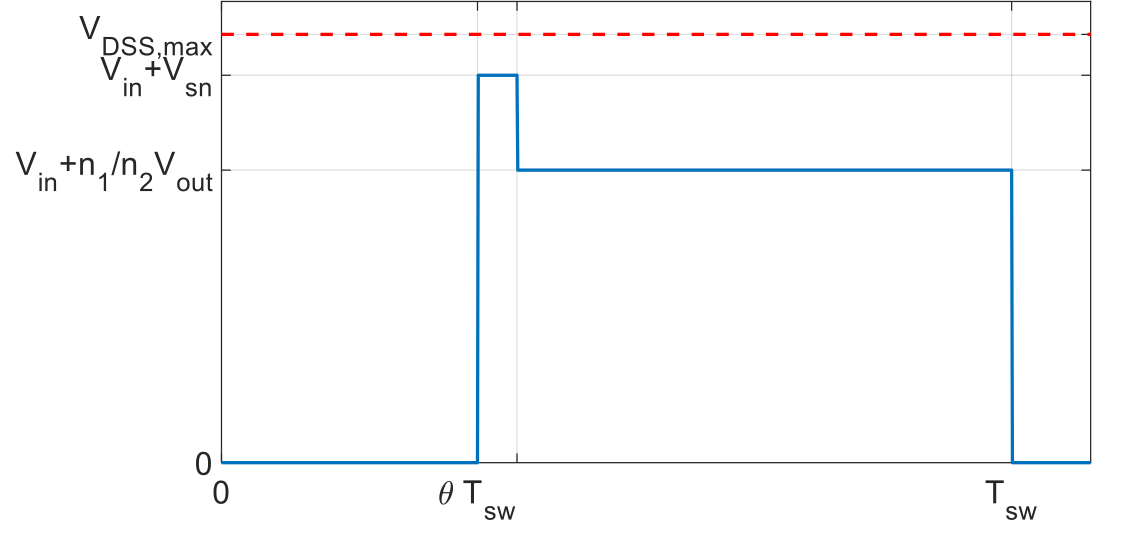
\includegraphics[width=0.7\textwidth]{Snubber2.png}
\end{figure}

$$R_{sn} = \frac{2 T_{sw} \alpha (\alpha - 1) \left(\frac{n_1}{n_2} V_{out} \right)^2}{L_f i^2_{mag,max}}$$
Avec généralement $\alpha \in \left[2, 2.5\right]$ 
$$C_{sn,min} = \frac{v_{sn,max}}{\Delta v_{sn,max} R_{sn} f_{sw}}$$
\end{solution}
\section{Superbuck  /6}

Soit le convertisseur suivant :

\begin{center}
	\begin{circuitikz}
		\draw[thick]
		(0,0) node[nmos, rotate = 90](nmos){}
		(nmos.D) to[short] (-2,0)
		(nmos.S) to[short] (5,0)
		(1.5,-2) to[diode] (1.5,0)
		(-1.5,-2) to[short] (1.5,-2)
		(-4,0) to[american voltage source,a=$V_{\mathrm{g}}$,right] (-4,-4) -- (5,-4)
		(5,0) to[R, l_=$R$, v^=$V$] (5,-4)
		(-4,0) to[L=$L$] (-2,0)
		(3,-4) to[C=$C$] (3,0)
		(0,-4) to[L=$L$] (0,-2)
		(-1.5,-2) to[C=$C$] (-1.5,0);
	\end{circuitikz}
\end{center}

Écrivez la matrice dynamique des états moyennés $\bm{A}$, en fonction du rapport cyclique.

\begin{solution}
  \begin{center}
        \begin{circuitikz}
                \draw[thick]
                (0,0) node[nmos, rotate = 90](nmos){}
                (nmos.D) to[short] (-2,0)
                (nmos.S) to[short] (5,0)
                (1.5,-2) to[diode] (1.5,0)
                (-1.5,-2) to[short] (1.5,-2)
                (-4,0) to[american voltage source,a=$V_{\mathrm{g}}$,right] (-4,-4) -- (5,-4)
                (5,0) to[R, l_=$R$$$] (5,-4)
                (-4,0) to[L=$L_1$,i>=$I_1$] (-2,0)
                (3,-4) to[C=$C_1$,v<=$V_1$] (3,0)
                (0,-4) to[L=$L_2$, i<=$I_2$] (0,-2)
                (-1.5,-2) to[C=$C_2$, v<=$V_2$] (-1.5,0);
        \end{circuitikz}
\end{center}
\begin{center}
\begin{tabular}{c|c|c}
&Ton&Toff\\
\hline
  $$I_{C_1} = \frac{C_1dV_1}{dt}& I_1 - I_2 -V_1/R& I_1 - I_2 - V_1/R\\
  I_{C_2} = \frac{C_2dV_2}{dt}& I_2 & I_1\\
  V_{L_1} = \frac{L_1dI_1}{dt}& V_g - V_1&V_g - (V_1 + V_2)\\
  V_{L_2} = \frac{L_2dI_2}{dt}& V_1 - V_2& V_1
\end{tabular}
\end{center}

  $$\begin{bmatrix}
  \frac{dV_1}{dt}\\
  \frac{dV_2}{dt}\\
  \frac{dI_1}{dt}\\
  \frac{dI_2}{dt}\\
\end{bmatrix}= 
  \begin{bmatrix}
    \frac{-1}{RC_1}& 0& \frac{1}{C_1}& \frac{-1}{C_1} \\
    0 & 0 & \frac{1-\theta}{C_2}& \frac{\theta}{C_2}\\
    \frac{-1}{L_1} & \frac{-1(1-\theta)}{L_1} 0 & 0\\
    \frac{1}{L_2} & \frac{-\theta}{L_2} & 0 &0
  \end{bmatrix}
  \begin{bmatrix}
   V_1\\
   V_2\\
   I_1\\
   I_2\\
  \end{bmatrix}$$
\end{solution}

\end{document}
